\documentclass{standalone}
\usepackage{apmep}
\usepackage{dcmaths}
\usepackage{dccornouaille}
\usepackage{dctikz}
\usepackage{dccours}
\usetikzlibrary{matrix,arrows,decorations.pathmorphing}
% l' unité
\newcommand{\myunit}{1 cm}
\tikzset{
    node style sp/.style={draw,circle,minimum size=\myunit},
    node style ge/.style={circle,minimum size=\myunit},
    arrow style mul/.style={draw,sloped,midway,fill=white},
    arrow style plus/.style={midway,sloped,fill=white},
}
\newcommand{\touchecalc}[1]{\fbox{#1}}
\begin{document}

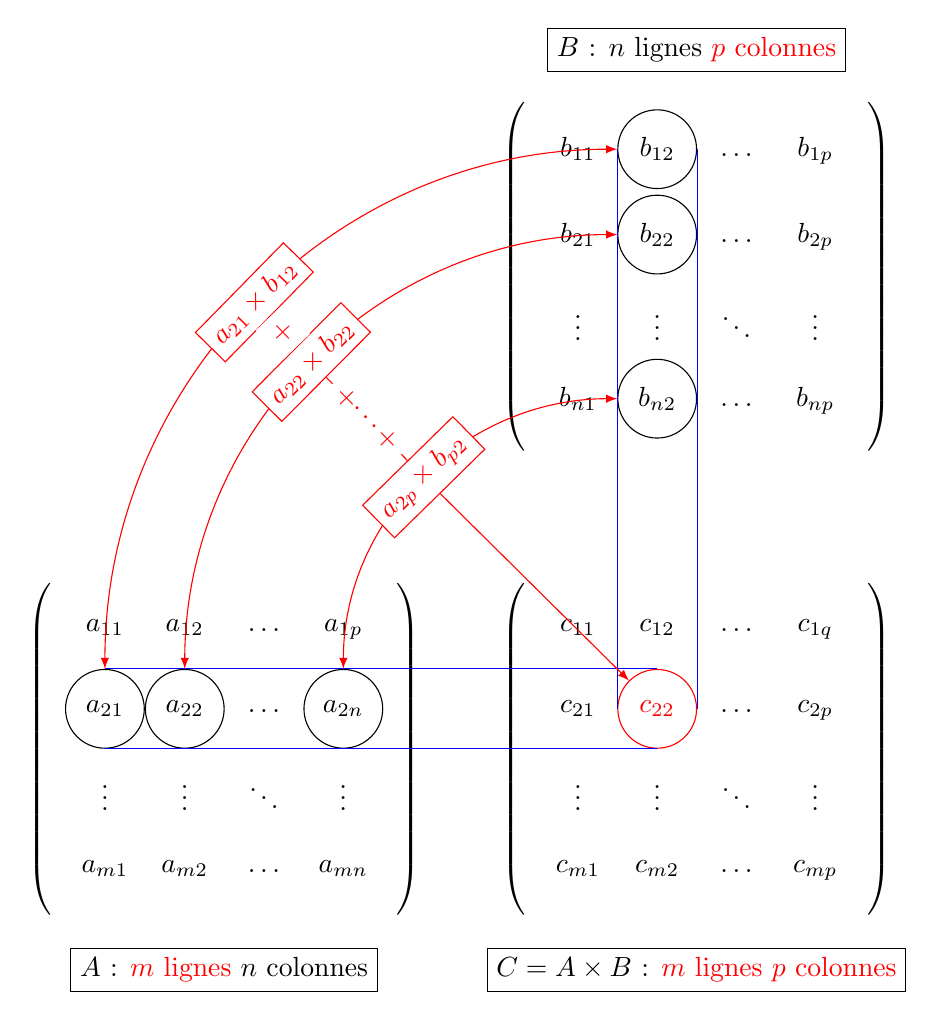
\begin{tikzpicture}[>=latex]
% les matrices
\matrix (A) [matrix of math nodes,%
nodes = {node style ge},%
left delimiter  = (,%
right delimiter = )] at (0,0)
{%
a_{11} & a_{12} & \ldots & a_{1p}  \\
\node[node style sp](A-2-1) {a_{21}};%
& \node[node style sp](A-2-2) {a_{22}};%
& \ldots%
& \node[node style sp](A-2-4) {a_{2n}}; \\
\vdots & \vdots & \ddots & \vdots  \\
a_{m1} & a_{m2} & \ldots & a_{mn}  \\
};
\node [draw,below=10pt] at (A.south)
{ $A$ : \textcolor{red}{$m$ lignes} $n$ colonnes};

\matrix (B) [matrix of math nodes,%
nodes = {node style ge},%
left delimiter  = (,%
right delimiter =)] at (6*\myunit,6*\myunit)
{%
b_{11} & \node[node style sp](B-1-2) {b_{12}};%
& \ldots & b_{1p}  \\
b_{21} & \node[node style sp](B-2-2) {b_{22}};%
& \ldots & b_{2p}  \\
\vdots & \vdots & \ddots & \vdots  \\
b_{n1} & \node[node style sp](B-4-2) {b_{n2}};%
& \ldots & b_{np}  \\
};
\node [draw,above=10pt] at (B.north)
{ $B$ : $n$ lignes \textcolor{red}{$p$ colonnes}};
% matrice résultat
\matrix (C) [matrix of math nodes,%
nodes = {node style ge},%
left delimiter  = (,%
right delimiter = )] at (6*\myunit,0)
{%
c_{11} & c_{12} & \ldots & c_{1q} \\
c_{21} & \node[node style sp,red](C-2-2) {c_{22}};%
& \ldots & c_{2p} \\
\vdots & \vdots & \ddots & \vdots \\
c_{m1} & c_{m2} & \ldots & c_{mp} \\
};
% les fleches
\draw[blue] (A-2-1.north) -- (C-2-2.north);
\draw[blue] (A-2-1.south) -- (C-2-2.south);
\draw[blue] (B-1-2.west)  -- (C-2-2.west);
\draw[blue] (B-1-2.east)  -- (C-2-2.east);
\draw[<->,red](A-2-1) to[in=180,out=90]
node[arrow style mul] (x) {$a_{21}\times b_{12}$} (B-1-2);
\draw[<->,red](A-2-2) to[in=180,out=90]
node[arrow style mul] (y) {$a_{22}\times b_{22}$} (B-2-2);
\draw[<->,red](A-2-4) to[in=180,out=90]
node[arrow style mul] (z) {$a_{2p}\times b_{p2}$} (B-4-2);
\draw[red,->] (x) to node[arrow style plus] {$+$} (y)%
to node[arrow style plus] {$+\raisebox{.5ex}{\ldots}+$} (z)%
to (C-2-2.north west);


\node [draw,below=10pt] at (C.south)
{$ C=A\times B$ : \textcolor{red}{$m$ lignes}  \textcolor{red}{$p$ colonnes}};

\end{tikzpicture}\end{document}